\section{Entanglement}

The concept of entanglement comes from the need of describing the difference of certain type of states respect to others. In particular, we can understand it by first defining a really simple type of state called separable that has the following form.
\dfn{Separable state}
{
    Taken a state $\ket{\psi}\in\mathcal{H}_1\otimes\mathcal{H}_2$ it's called separable if $\exists \ket{\phi_1}\in \mathcal{H}_1, \ket{\phi_2} \in \mathcal{H}_2$ so that we can write
    \begin{equation}
        \ket{\psi} = \ket{\phi_1}\otimes\ket{\phi_2}.
    \end{equation}
}
\noindent
This type of states are really simple since we can decompose them into simpler once and work with them. To make an example we can see how the state $(\ket{01} + \ket{00})/\sqrt{2}$ is a separable one since
\begin{equation}
    \frac{\ket{01} + \ket{00}}{\sqrt{2}} = \ket{0}\left( \frac{\ket{0} + \ket{1}}{\sqrt{2}} \right),
\end{equation}
holds true and so can be decomposed. Nevertheless, we shall not go much further to find out more complex states that cannot be decomposed for which we need to work in the higher dimensional space like the Bell's state $(\ket{01} + \ket{10})/\sqrt{2}$. Those are entangled states, whose definition is therefore really simple as.
\dfn{Entangled states}
{
    \label{def:Entangl}
    A state $\ket{\psi}\in\mathcal{H}_1\otimes\mathcal{H}_2$ it's called entangled if it's not separable.
}
\noindent
Therefore, the mathematical definition of entanglement seems really simple, but the physical consequences are not, and we shall see together why this is one of the main powers of QC.

\ex{}
{
    To make an example of how powerful the entanglement can be we can see how in theory we can transport the information of two bits, so $00$, $01$, $10$ or $11$, transmitting only one qubit. The idea is that two people, Alice and Bob, posses two qubit that are entangled in the following Bell state
    \begin{equation}
        \ket{\psi^+} = \frac{\ket{00} + \ket{11}}{\sqrt{2}},
    \end{equation}
    then Alice can perform one of four operations on it's qubit based on what wants to transmit to Bob. In particular the following choices can be made
    \begin{align*}
        &\text{Operation}               &\text{Final state}\\
        &\ket{00} \to \mathbb{1}        &\ket{\psi^+}\hspace{0.4cm}\\
        &\ket{01} \to Z                 &\ket{\psi^-}\hspace{0.4cm}\\
        &\ket{10} \to X                 &\ket{\phi^+}\hspace{0.4cm}\\
        &\ket{11} \to iY                &\ket{\phi^-}\hspace{0.4cm}
    \end{align*}
    So, based on the information that we want to send we have performed an operation of the Alice qubit to obtain a different Bell state. Then, Alice only need to send the qubit to Bob which need to perform a two qubit measure using the Bell's base and the state that will obtain will correspond to the selected two bit information obtained with the transport of only one qubit.
}

\nt
{
    This definition of Entanglement is not really the most general one that can be used. In fact, the Def. (\ref{def:Entangl}) it's a specific one called bi-entanglement since only two Hilbert spaces are counted, but the most general called n-entanglement count for $\ket{\psi}\in \bigotimes_{i=1}^n \mathcal{H}_i$. Nevertheless, for QC application only the bi-entanglement plays an important role.
}

\subsection{Quantum teleportation}

The first real important application of entanglement that we will see it's the quantum protocol for the quantum teleportation of information. Basically we want to teleport a quantum state from one qubit to another, so that no matter is transported to one place to another but only the state of the qubits is changed transporting information. Also, at first site one can also think that the cloning theorem would be violated in a situation of this type, but that is not the case, and we will see why.
\begin{figure}[b]
    \centering
    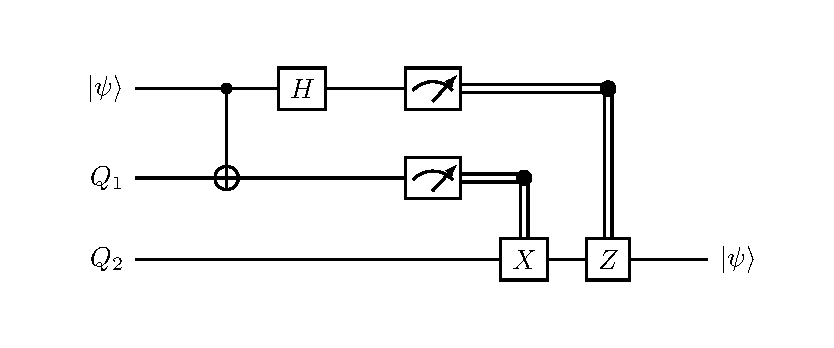
\includegraphics[width=0.8\textwidth]{Immagini/QuanTeleport.pdf}
    \caption
    {
        Quantum teleportation circuit for a quantum computer, see how it involves the measuring of two qubit to control two operations.
    }
    \label{fig:QuanTeleport}
\end{figure}

The circuit that is used in order to perform the teleportation protocol is reported in \figref{fig:QuanTeleport}, and consist in the use of two qubit in order to transport a general state $\ket{\psi} = a\ket{0} + b\ket{1}$ into one of those qubit. Thus, we want to understand how this is possible in general, and to do that let's pretend that the two qubit $\ket{\psi}$ and $Q_1$ are in possession of Alice, while $Q_2$ is with Bob. We will need that the two qubit $Q_1$, $Q_2$ are entangled in a $\ket{\psi^+}$ Bell state, then we can place them at whatever distance, so that Alice and Bob can be also on different planets. In this situation Alice will perform a series of operation on her qubit starting with a CNOT, to understand what this operation will do on the system we need first to look at the state of the hole three qubit, which will be
\begin{equation}
    \ket{\psi Q_1Q_2} = \left( a\ket{0} + b\ket{1} \right)\left( \frac{\ket{00} + \ket{11}}{\sqrt{2}} \right) = \frac{1}{\sqrt{2}}\left[ a\ket{000} + a\ket{011} + b\ket{100} + b\ket{111} \right].
\end{equation}
Then we can easily perform the CNOT on the first two qubit ending up in the following state
\begin{equation}
    \frac{1}{\sqrt{2}}\left[ a\ket{000} + a\ket{011} + b\ket{110} + b\ket{101} \right],
\end{equation}
on which the Hadamart tranformation is applied on the first qubit, which we shall remember that transforms $\ket{0}$ in $\ket{+}$ and $\ket{1}$ in $\ket{-}$. Therefore, we will have the following form
\begin{equation}
    \frac{1}{2}\left[ a\ket{000} + a\ket{100} + a\ket{011} + a\ket{111} + b\ket{010} - b\ket{110} + b\ket{001} - b\ket{101} \right],
\end{equation}
which can be rewritten by seeing how inside it four separable states can be found out, having
\begin{equation}
    \frac{1}{2}\left[ \ket{00}\left( a\ket{0} + b\ket{1} \right) + \ket{01}\left( a\ket{1} + b\ket{0} \right) + \ket{10}\left( a\ket{0} - b\ket{1} \right) + \ket{11}\left( a\ket{1} - b\ket{0} \right) \right].
\end{equation}
At first sight this state may seem nothing special, but if the states inside parentheses are inspected one could find out different forms of $\ket{\psi}$ obtaining
\begin{equation}
    \frac{1}{2}\left[ \ket{00}\left( \ket{\psi} \right) + \ket{01}\left( X\ket{\psi} \right) + \ket{10}\left( Z\ket{\psi} \right) + \ket{11}\left( XZ\ket{\psi} \right) \right].
\end{equation}
We have so created a state where the two qubit state given by Alice's couple is entangled to the qubit of Bob, which will poses the $\ket{\psi}$ state up to two transformation based on the Alice's values. Therefore, if Alice measure it's two qubit and refers the outcomes to Bob, he can perform the right operations to obtain at the end the final state $\ket{\psi}$ on his qubit. An operation that inside the circuit is described by the two classical controls and can be seen gives the right result keeping in mind that $X^2 = Z^2 = \mathbb{1}$.

Thus, using this protocol a general state $\ket{\psi}$ can be transferred into another qubit at whatever distance without limitations. In fact, the circuit has been performed in several occasions starting from a teleportation distance of some centimeters to the experiment of Anton Zellinger that performed it at nearly one kilometer of distance inside Vienna. Today we are able to transfer states from hearth to satellite, but still this phenomenon result in being quite strange at first sight. Perhaps, as was told earlier, one can say that this \textbf{phenomenon contradicts Thm. (\ref{thm:cloning})} with the coping of a general state into another one. This is a wrong affirmation, since the non-cloning theorem tells that the following operation doesn't exist
\begin{equation}
    \mathcal{U}(\ket{\psi}\otimes\ket{s}) = \ket{\psi}\otimes\ket{\psi},
\end{equation}
while here the starting states have been measured by Alice, meaning that they have collapsed having a result more similar to
\begin{equation}
    \mathcal{U}(\ket{\psi}\otimes\ket{Q_1}\otimes\ket{Q_2}) = \ket{00}\otimes\ket{\psi}.
\end{equation}
Where $\ket{00}$ is only one of the four possible final result obtained. Another apparent contradiction that can be found out inside the teleportation protocol is the fact that \textbf{information seem to pass from one qubit to another faster than the speed of light}. That can't obviously be possible, since relativity forbid it, and in fact that is not the case. The two classical controls that are used inside the circuit solve the problem since in order to obtain the copied state inside $Q_2$ I first need Alice to transmit the result of the measurements to Bob and that classical exchange of information take times.